\documentclass[12pt,a4paper]{article}
\usepackage[left=15mm,right=15mm,top=14mm,bottom=20mm,footskip=10mm]{geometry}
\usepackage{iftex}
\ifPDFTeX
  \usepackage[T5]{fontenc}
  \usepackage[utf8]{inputenc}
  \usepackage{mathptmx}
\else
  \usepackage{fontspec}
  \setmainfont{Times New Roman}
\fi
\usepackage{amsmath,amssymb}
\usepackage{fix-cm}
\usepackage{tikz}
\usetikzlibrary{arrows.meta}
\usepackage{tcolorbox}
\usepackage{fancyhdr}
\usepackage{lastpage}
\usepackage{tabularx}
\definecolor{sectionpurple}{RGB}{155,42,143}
\definecolor{notebackground}{RGB}{229,240,245}
\definecolor{noteborder}{RGB}{255,55,55}
\setlength{\parindent}{0pt}
\setlength{\parskip}{2pt}
\setlength{\headheight}{15pt}
\pagestyle{fancy}
\fancyhf{}
\renewcommand{\headrulewidth}{0pt}
\renewcommand{\footrulewidth}{0.4pt}
\fancyfoot[L]{\fontsize{8.5}{10}\selectfont
  Biên soạn: \textbf{Nguyễn Anh Dũng}}
\fancyfoot[R]{\fontsize{8.5}{10}\selectfont
  Trang \thepage/\pageref{LastPage} -- Đề TDMXX01A}
\newtcolorbox{notebox}{colback=notebackground,colframe=noteborder,
  boxrule=0.8pt,arc=2pt,left=8pt,right=8pt,top=4pt,bottom=4pt,
  before skip=4pt,after skip=4pt}
\newcommand{\question}[2][TDM21]{%
  \par\addvspace{5pt}\noindent
  \textbf{\textcolor{sectionpurple}{Câu #2:} \textcolor{noteborder}{[#1]}}\enspace
}
\newcommand{\answerlabel}[1]{\textbf{\textcolor{sectionpurple}{#1.}}}
\newcommand{\fourchoices}[4]{%
  \par\nobreak\smallskip
  \begin{tabular*}{\linewidth}{@{}l@{\extracolsep{\fill}}lll@{}}
    \answerlabel{A} #1 & \answerlabel{B} #2 & \answerlabel{C} #3 & \answerlabel{D} #4
  \end{tabular*}\par
}
\newcommand{\twochoices}[4]{%
  \par\nobreak\smallskip
  \begin{tabularx}{\linewidth}{@{}>{\raggedright\arraybackslash}X>{\raggedright\arraybackslash}X@{}}
    \answerlabel{A} #1 & \answerlabel{B} #2 \\[2pt]
    \answerlabel{C} #3 & \answerlabel{D} #4
  \end{tabularx}\par
}


\newcommand{\homeworkgraph}[2]{%
  \begin{notebox}
  \centering
  \begin{tikzpicture}[x=0.38cm,y=0.48cm,
    every node/.style={font=\fontsize{11.5}{14}\selectfont}]
    \draw[thin,-{Stealth[length=4pt]}] ({#1-4},0) -- ({#2+8},0) node[below] {$x$};
    \draw[thin,-{Stealth[length=4pt]}] (0,-1.9) -- (0,3.8) node[right] {$y$};
    \draw[thin,densely dashed] (#1,0) -- (#1,3);
    \draw[thin,densely dashed] (#2,0) -- (#2,-1.5);
    \draw[black,thin]
      ({#1-3},-1.1) .. controls ({#1-2},1.1) and ({#1-1},3) .. (#1,3)
      .. controls ({#1+2},3) and ({#2-2},-1.5) .. (#2,-1.5)
      .. controls ({#2+1.5},-1.5) and ({#2+3},1.4) .. ({#2+4},3.3);
    \fill (#1,3) circle (1.3pt);
    \fill (#1,0) circle (1.3pt);
    \fill (#2,0) circle (1.3pt);
    \fill (#2,-1.5) circle (1.3pt);
    \node[below] at (#1,0) {$#1$};
    \node[above] at (#2,0) {$#2$};
    \node[below left] at (0,0) {$O$};
    \node[right] at ({#2+3.6},2.5) {$f(x)$};
  \end{tikzpicture}
  \end{notebox}%
}


\newcommand{\shortanswer}{%
  \par\nobreak\hfill
  
\begin{tikzpicture}
    \node[draw=noteborder,fill=notebackground,line width=0.8pt,
      rounded corners=2pt,minimum width=24mm,minimum height=6mm,inner sep=0pt] {};
  \end{tikzpicture}\par
}

\begin{document}
\fontsize{12}{15}\selectfont

{\centering
\textbf{ĐỀ TDMXX01A}\par
\textbf{CƠ BẢN VỀ ĐƠN ĐIỆU CỦA HÀM SỐ}\par
{\fontsize{10.5}{13}\selectfont\itshape
Form đề chuẩn bám sát BGD2025 -- Thời gian làm bài \textbf{90 phút}\par}}

\textbf{Phần I. Câu trắc nghiệm nhiều phương án lựa chọn.}
Thí sinh trả lời từ câu 1 đến câu 12. Mỗi câu hỏi thí sinh chỉ chọn một phương án.

\question{1} Cho bảng biến thiên của hàm số $f(x)$ như hình vẽ. Hàm số $f(x)$ đồng biến trên
\begin{notebox}
\centering
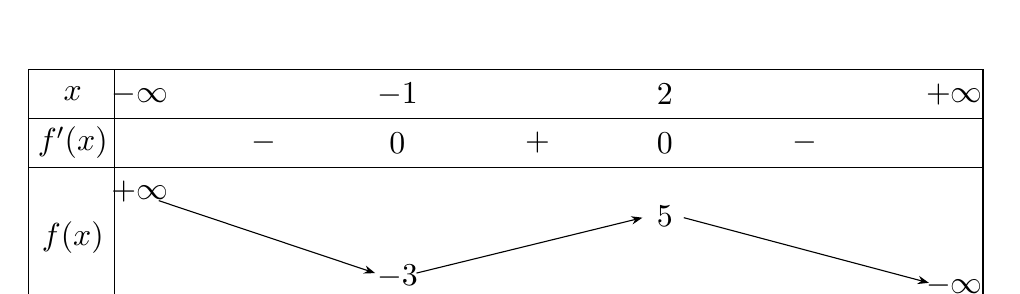
\begin{tikzpicture}[x=\linewidth/15,y=-22pt,
  every node/.style={font=\fontsize{11.5}{14}\selectfont}]
  \draw[thin] (0,-0.4) rectangle (15,3.5);
  \draw[thin] (1.35,-0.4) -- (1.35,3.5);
  \draw[thin] (0,0.4) -- (15,0.4);
  \draw[thin] (0,1.2) -- (15,1.2);
  \node at (0.7,0) {$x$};
  \node at (0.7,0.8) {$f'(x)$};
  \node at (0.7,2.35) {$f(x)$};
  \foreach \position/\entry in {1.75/{-\infty},5.8/{-1},10/{2},14.55/{+\infty}}
    \node at (\position,0) {$\entry$};
  \foreach \position/\entry in {3.7/{-},5.8/{0},8/{+},10/{0},12.2/{-}}
    \node at (\position,0.8) {$\entry$};
  \node at (1.75,1.6) {$+\infty$};
  \node at (5.8,3) {$-3$};
  \node at (10,2) {$5$};
  \node at (14.55,3.15) {$-\infty$};
  \draw[thin,-{Stealth[length=4pt]}] (2.05,1.75) -- (5.45,2.94);
  \draw[thin,-{Stealth[length=4pt]}] (6.1,2.94) -- (9.65,2.03);
  \draw[thin,-{Stealth[length=4pt]}] (10.3,2.03) -- (14.15,3.1);
\end{tikzpicture}
\end{notebox}
\fourchoices{$(-1;2)$}{$(-3;5)$}{$(-\infty;-1)$}{$(2;+\infty)$}

\question{2} Cho hàm số $f(x)$ liên tục và xác định trên $\mathbb{R}$, có bảng xét dấu đạo hàm như hình vẽ. Hàm số $f(x)$ đồng biến trên
\begin{notebox}
\centering
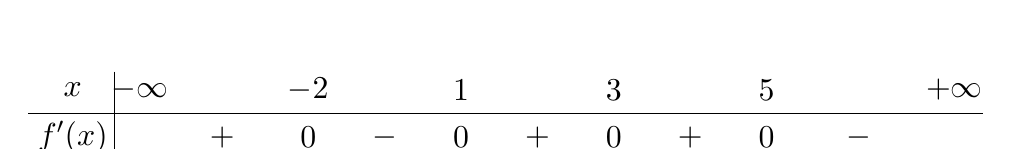
\begin{tikzpicture}[x=\linewidth/15,y=-19pt,
  every node/.style={font=\fontsize{11.5}{14}\selectfont}]
  \draw[thin] (0,0.45) -- (15,0.45);
  \draw[thin] (1.35,-0.35) -- (1.35,1.25);
  \node at (0.7,0) {$x$};
  \node at (0.7,0.9) {$f'(x)$};
  \foreach \position/\entry in {1.75/{-\infty},4.4/{-2},6.8/{1},9.2/{3},11.6/{5},14.55/{+\infty}}
    \node at (\position,0) {$\entry$};
  \foreach \position/\entry in {3.05/{+},4.4/{0},5.6/{-},6.8/{0},8/{+},9.2/{0},10.4/{+},11.6/{0},13.05/{-}}
    \node at (\position,0.9) {$\entry$};
\end{tikzpicture}
\end{notebox}
\twochoices{$(-\infty;-2)$ và $(5;+\infty)$.}{$(-\infty;-2)$ và $(1;5)$.}
  {$(3;+\infty)$}{$(-2;1)$ và $(5;+\infty)$.}

\question{3} Hàm số nào dưới đây đồng biến trên tập xác định của nó?
\fourchoices{$y=\dfrac{x-2}{x+1}$}{$y=x^4+2x^2+2$}{$y=-\sin x$}{$y=x^5+6x-1$}

\question{4} Hàm số $f(x)=-x^3+12x$ nghịch biến trên khoảng
\fourchoices{$(-\infty;-2)$}{$(-2;2)$}{$(-2;+\infty)$}{$\mathbb{R}$}

\question{5} Hàm số $y=\dfrac{x-2}{x+1}$
\twochoices{nghịch biến trên từng khoảng xác định.}{đồng biến trên tập xác định.}
  {đồng biến trên $(-\infty;-1)\cup(-1;+\infty)$.}{đồng biến trên từng khoảng xác định.}

\question{6} Hàm số $y=\dfrac{3x+1}{x-2}$
\twochoices{có đạo hàm luôn âm trên tập xác định.}{nghịch biến trên tập xác định.}
  {đồng biến trên $(-\infty;2)\cup(2;+\infty)$.}{đồng biến trên từng khoảng xác định.}

\question{7} Hàm số $y=f(x)=\dfrac{x^2-3x+3}{x-2}$ đồng biến trên khoảng
\fourchoices{$(2;+\infty)$}{$(1;2)$}{$(-\infty;1)$}{$(1;3)$}

\smallskip
{\fontsize{9}{11}\selectfont\itshape
\textsuperscript{*}Ảnh gốc thiếu nội dung sau chữ ``và'' ở phương án C, Câu 2.\par}


\newpage

\question{8} Hàm số $y=-x^3+3x^2$ đồng biến trên
\fourchoices{$(0;1)$}{$(1;3)$}{$(-\infty;0)$}{$(2;+\infty)$}

\question{9} Cho hàm số $y=f(x)$ có đồ thị như hình vẽ bên dưới.
Hàm số $y=-6f(x)+2026$ đồng biến trên khoảng
\homeworkgraph{-3}{5}
\fourchoices{$(-\infty;-3)$}{$(-3;5)$}{$(-\infty;+\infty)$}{$(5;+\infty)$}

\question{10} Cho hàm số $y=f(x)$ có đồ thị như hình vẽ bên dưới.
Hàm số $y=5f(x)-1$ nghịch biến trên khoảng nào dưới đây?
\homeworkgraph{-4}{7}
\fourchoices{$(-4;7)$}{$(-\infty;-4)$}{$(1;12)$}{$(-20;35)$}

\question{11} Hàm số $y=x^2-2\cos x$ đồng biến trên khoảng
\fourchoices{$(0;+\infty)$}{$(-\infty;0)$}{$\left(-\dfrac{\pi}{2};\dfrac{\pi}{2}\right)$}{$(-\pi;0)$}

\question{12} Hàm số $y=3x^2-\sin 2x$ nghịch biến trên khoảng
\fourchoices{$(0;+\infty)$}{$\left(-\dfrac{\pi}{2};\dfrac{\pi}{3}\right)$}{$(-\infty;0)$}{$\left(\pi;\dfrac{3\pi}{2}\right)$}

\par\addvspace{7pt}
\textbf{Phần II. Câu trắc nghiệm đúng sai.}
Thí sinh trả lời từ câu 13 đến câu 16. Trong mỗi ý \textbf{a), b), c), d)} ở mỗi câu,
thí sinh chọn \textbf{đúng} hoặc \textbf{sai}.

\question[TDM32]{13} Cho hàm số $f(x)=ax^2+bx+c$, với các hệ số thực $a,b,c$.
Hỏi trong các mệnh đề dưới đây, mệnh đề nào \textbf{đúng}, mệnh đề nào \textbf{sai}?

\begin{notebox}
\renewcommand{\arraystretch}{1.5}
\setlength{\tabcolsep}{5pt}
\begin{tabularx}{\linewidth}{|>{\bfseries\color{sectionpurple}}c|>{\raggedright\arraybackslash}X|c|c|}
\hline
\multicolumn{2}{|c|}{\textbf{\textcolor{sectionpurple}{Mệnh đề}}}
& \textbf{\textcolor{sectionpurple}{Đ}} & \textbf{\textcolor{sectionpurple}{S}} \\
\hline
a & Nếu $a>0$ thì hàm số $f(x)$ đồng biến trên khoảng $\left(-\dfrac{b}{2a};+\infty\right)$.
& $\bigcirc$ & $\bigcirc$ \\[3pt]
\hline
b & Nếu $a<0$ thì hàm số $f(x)$ nghịch biến trên khoảng $\left(-\infty;-\dfrac{b}{2a}\right)$.
& $\bigcirc$ & $\bigcirc$ \\[3pt]
\hline
c & Hàm số $f(x)$ đồng biến trên $\mathbb{R}$ khi và chỉ khi $\begin{cases}a=0\\b>0.\end{cases}$
& $\bigcirc$ & $\bigcirc$ \\[3pt]
\hline
d & Hàm số $f(x)$ nghịch biến trên $(2;+\infty)$ khi và chỉ khi $\begin{cases}a=0\\b<0.\end{cases}$
& $\bigcirc$ & $\bigcirc$ \\[3pt]
\hline
\end{tabularx}
\end{notebox}


\newpage

\question[TDM31]{14} Cho hàm số $f(x)$ xác định trên $\mathbb{R}$, có đồ thị hàm số $y=f'(x)$ như hình vẽ bên dưới.
Hãy chọn tính đúng sai của các nhận xét sau:

\begin{notebox}
{\centering
\begin{tikzpicture}[x=0.58cm,y=0.58cm,
  every node/.style={font=\fontsize{11.5}{14}\selectfont}]
  \draw[thin,-{Stealth[length=4pt]}] (-9.5,0) -- (6,0) node[below] {$x$};
  \draw[thin,-{Stealth[length=4pt]}] (0,-3.1) -- (0,4.1) node[left] {$y$};
  \draw[thin,densely dashed] (-5,0) -- (-5,-2.6);
  \draw[thin,densely dashed] (2,0) -- (2,2.5);
  \draw[black,thin]
    (-8.4,3.7) .. controls (-8,2.1) and (-7.4,0.5) .. (-7,0)
    .. controls (-6.4,-1.4) and (-5.7,-2.6) .. (-5,-2.6)
    .. controls (-4,-2.6) and (-2.7,0) .. (-2,0)
    .. controls (-1.6,0) and (-1.7,-2.4) .. (-1.2,-2.4)
    .. controls (-0.8,-2.4) and (-0.3,-0.8) .. (0,0)
    .. controls (0.6,1.3) and (1.4,2.5) .. (2,2.5)
    .. controls (2.4,2.5) and (2.75,0.6) .. (3,0)
    .. controls (3.4,-0.8) and (3.9,-1.8) .. (4.4,-2.6);
  \foreach \abscissa in {-7,-5,-2,2,3}
    \fill (\abscissa,0) circle (1.3pt);
  \fill (-5,-2.6) circle (1.3pt);
  \fill (2,2.5) circle (1.3pt);
  \node[below left] at (-7,0) {$-7$};
  \node[below left] at (-5,0) {$-5$};
  \node[below left] at (-2,0) {$-2$};
  \node[above left] at (0,0) {$O$};
  \node[below] at (2,0) {$2$};
  \node[above right] at (3,0) {$3$};
  \node[right] at (3,2.1) {$f'(x)$};
\end{tikzpicture}\par}
\smallskip
\renewcommand{\arraystretch}{1.45}
\setlength{\tabcolsep}{5pt}
\begin{tabularx}{\linewidth}{|>{\bfseries\color{sectionpurple}}c|>{\raggedright\arraybackslash}X|c|c|}
\hline
\multicolumn{2}{|c|}{\textbf{\textcolor{sectionpurple}{Mệnh đề}}}
& \textbf{\textcolor{sectionpurple}{Đ}} & \textbf{\textcolor{sectionpurple}{S}} \\
\hline
a & Hàm số $f(x)$ nghịch biến trên khoảng $(-\infty;-5)$.
& $\bigcirc$ & $\bigcirc$ \\
\hline
b & Hàm số $f(x)$ nghịch biến trên khoảng $(-7;0)$.
& $\bigcirc$ & $\bigcirc$ \\
\hline
c & Hàm số $f(x)$ đồng biến trên khoảng $(a;b)\subset(0;3)$, với $(a;b)\neq\varnothing$.
& $\bigcirc$ & $\bigcirc$ \\
\hline
d & Có đúng $3$ giá trị nguyên của $a$ để $f(x)$ nghịch biến trên khoảng $(a+4;16-a^2)$.
& $\bigcirc$ & $\bigcirc$ \\
\hline
\end{tabularx}
\end{notebox}

\question[TDM32]{15} Cho hàm số bậc ba $f(x)=ax^3+bx^2+cx+d$, với các hệ số thực $a,b,c,d$ có $a\neq 0$.
Hỏi trong các mệnh đề dưới đây, mệnh đề nào \textbf{đúng}, mệnh đề nào \textbf{sai}?

\begin{notebox}
\renewcommand{\arraystretch}{1.5}
\setlength{\tabcolsep}{5pt}
\begin{tabularx}{\linewidth}{|>{\bfseries\color{sectionpurple}}c|>{\raggedright\arraybackslash}X|c|c|}
\hline
\multicolumn{2}{|c|}{\textbf{\textcolor{sectionpurple}{Mệnh đề}}}
& \textbf{\textcolor{sectionpurple}{Đ}} & \textbf{\textcolor{sectionpurple}{S}} \\
\hline
a & Hàm số $f(x)$ đồng biến trên $\mathbb{R}$ khi và chỉ khi $b^2-3ac\leq 0$.
& $\bigcirc$ & $\bigcirc$ \\[2pt]
\hline
b & Hàm số $f(x)$ nghịch biến trên $\mathbb{R}$ khi và chỉ khi $\begin{cases}a<0\\b^2-3ac\leq 0.\end{cases}$
& $\bigcirc$ & $\bigcirc$ \\[2pt]
\hline
c & Với $a>0$, hàm số $f(x)$ nghịch biến trên $(\alpha;\beta)$ khi và chỉ khi $\begin{cases}f'(\alpha)\leq 0\\f'(\beta)\leq 0.\end{cases}$
& $\bigcirc$ & $\bigcirc$ \\[2pt]
\hline
d & Với $a<0$, hàm số $f(x)$ đồng biến trên $(\alpha;\beta)$ khi và chỉ khi $\begin{cases}f'(\alpha)\leq 0\\f'(\beta)\leq 0.\end{cases}$
& $\bigcirc$ & $\bigcirc$ \\[2pt]
\hline
\end{tabularx}
\end{notebox}

\question[TDM32]{16} Cho hàm số trùng phương $f(x)=x^4+bx^2+c$, với các hệ số thực $b,c$ có $a\neq 0$.
Hỏi trong các mệnh đề dưới đây, mệnh đề nào \textbf{đúng}, mệnh đề nào \textbf{sai}?

\begin{notebox}
\renewcommand{\arraystretch}{1.5}
\setlength{\tabcolsep}{5pt}
\begin{tabularx}{\linewidth}{|>{\bfseries\color{sectionpurple}}c|>{\raggedright\arraybackslash}X|c|c|}
\hline
\multicolumn{2}{|c|}{\textbf{\textcolor{sectionpurple}{Mệnh đề}}}
& \textbf{\textcolor{sectionpurple}{Đ}} & \textbf{\textcolor{sectionpurple}{S}} \\
\hline
a & Hàm số $f(x)$ đồng biến trên $\mathbb{R}$ với mọi $b,c\in\mathbb{R}$.
& $\bigcirc$ & $\bigcirc$ \\
\hline
b & Hàm số $f(x)$ nghịch biến trên $(0;+\infty)$ khi và chỉ khi $b\geq 0$.
& $\bigcirc$ & $\bigcirc$ \\
\hline
c & Hàm số $f(x)$ nghịch biến trên $(0;2)$ khi và chỉ khi $b\leq -8$.
& $\bigcirc$ & $\bigcirc$ \\
\hline
d & Hàm số $f(x)$ đồng biến trên $(-3;0)$ khi và chỉ khi $b\leq -9$.
& $\bigcirc$ & $\bigcirc$ \\
\hline
\end{tabularx}
\end{notebox}


\newpage

\textbf{Phần III. Câu trắc nghiệm trả lời ngắn.}
Thí sinh trả lời từ câu 17 đến câu 22.

\question[TDM31]{17} Cho hàm số $y=f(x)$ có biểu thức đạo hàm
$f'(x)=(x+3)^2(x-1)^3(x-2)$ với $\forall x\in\mathbb{R}$.
Hàm số nghịch biến trên khoảng $(\alpha;\beta)$. Giá trị lớn nhất của biểu thức $(\beta-\alpha)$ tương ứng bằng:
\shortanswer

\question[TDM31]{18} Cho hàm số $y=f(x)=x^4-2x^2$.
Biết rằng hàm số nghịch biến trên khoảng $\left(0;\dfrac{m}{6}\right)$.
Hỏi có bao nhiêu giá trị nguyên của $m$ thoả mãn?
\shortanswer

\question[TDM32]{19} Cho hàm số $y=f(x)$ có đồ thị như hình vẽ bên dưới.
Gieo ngẫu nhiên một con súc sắc cân đối đồng chất và gọi $b$ là số chấm xuất hiện.
Hãy tính xác suất để hàm số $f(x)$ đồng biến trên khoảng $(2b-5;b-2)$
(làm tròn kết quả đến hàng phần trăm)?

\begin{notebox}
\centering
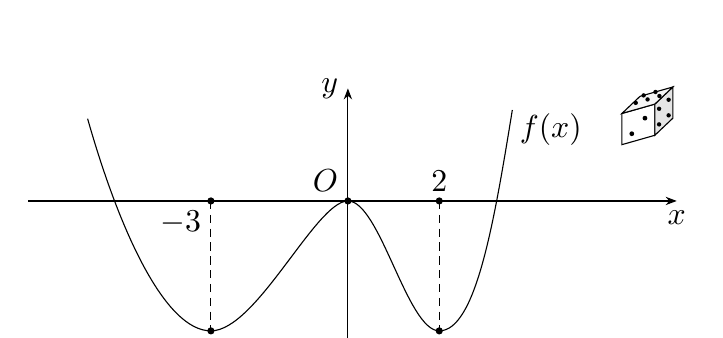
\begin{tikzpicture}[x=0.58cm,y=0.55cm,
  every node/.style={font=\fontsize{11.5}{14}\selectfont}]
  \draw[thin,-{Stealth[length=4pt]}] (-7,0) -- (7.2,0) node[below] {$x$};
  \draw[thin,-{Stealth[length=4pt]}] (0,-3.45) -- (0,2.6) node[left] {$y$};
  \draw[thin,densely dashed] (-3,0) -- (-3,-3);
  \draw[thin,densely dashed] (2,0) -- (2,-3);
  \draw[black,thin]
    (-5.7,1.9) .. controls (-5,-0.7) and (-4,-3) .. (-3,-3)
    .. controls (-2,-3) and (-0.7,0) .. (0,0)
    .. controls (0.7,0) and (1.3,-3) .. (2,-3)
    .. controls (2.8,-3) and (3.2,-0.5) .. (3.6,2.1);
  \foreach \abscissa in {-3,0,2}
    \fill (\abscissa,0) circle (1.3pt);
  \fill (-3,-3) circle (1.3pt);
  \fill (2,-3) circle (1.3pt);
  \node[below left] at (-3,0) {$-3$};
  \node[above left] at (0,0) {$O$};
  \node[above] at (2,0) {$2$};
  \node[right] at (3.55,1.65) {$f(x)$};
  \begin{scope}[shift={(6,1.3)},scale=0.72]
    \draw[thin,fill=white] (0,0) -- (1,0.3) -- (1,1.3) -- (0,1) -- cycle;
    \draw[thin,fill=gray!20] (1,0.3) -- (1.55,0.85) -- (1.55,1.85) -- (1,1.3) -- cycle;
    \draw[thin,fill=gray!8] (0,1) -- (0.55,1.55) -- (1.55,1.85) -- (1,1.3) -- cycle;
    \fill (0.3,0.35) circle (1.2pt);
    \fill (0.7,0.85) circle (1.2pt);
    \foreach \pipx/\pipy in {1.13/0.65,1.42/0.94,1.13/1.15,1.42/1.44}
      \fill (\pipx,\pipy) circle (1.1pt);
    \foreach \pipx/\pipy in {0.42/1.34,0.66/1.58,0.78/1.45,1.02/1.69,1.14/1.56}
      \fill (\pipx,\pipy) circle (1.1pt);
  \end{scope}
\end{tikzpicture}
\end{notebox}
\shortanswer

\question[TDM32]{20} Cho hàm số $y=f(x)=x^3-6x^2+9x-1$.
Hỏi có tất cả bao nhiêu giá trị nguyên của tham số $a$ để hàm số $f(x)$ nghịch biến trên $(3a-1;a^2+2)$?
\shortanswer

\question[TDM32]{21} Cho hàm số $f(x)$ có biểu thức đạo hàm $f'(x)=(x-1)(x-5)$.
Hỏi có tất cả bao nhiêu bộ số nguyên $(a;b)$ sao cho hàm số $f(x)$ nghịch biến trên khoảng $(a;b)$?
\shortanswer

\question[TDM32]{22} Cho hàm số $y=f(x)$ có đồ thị đạo hàm $y=f'(x)$ như hình vẽ bên dưới.
Hỏi có tất cả bao nhiêu khoảng có các đầu mút là những số nguyên mà hàm số $f(x)$ đồng biến trên đó?

\begin{notebox}
\centering
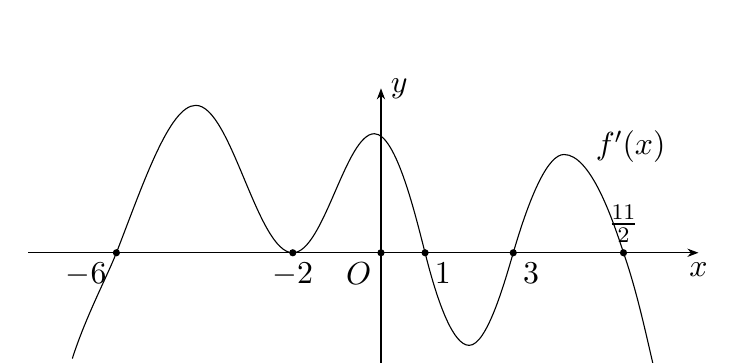
\begin{tikzpicture}[x=0.56cm,y=0.48cm,
  every node/.style={font=\fontsize{11.5}{14}\selectfont}]
  \draw[thin,-{Stealth[length=4pt]}] (-8,0) -- (7.2,0) node[below] {$x$};
  \draw[thin,-{Stealth[length=4pt]}] (0,-3.25) -- (0,4.35) node[right] {$y$};
  \draw[black,thin]
    (-7,-2.8) .. controls (-6.7,-1.7) and (-6.2,-0.6) .. (-6,0)
    .. controls (-5.4,1.8) and (-4.8,3.9) .. (-4.2,3.9)
    .. controls (-3.4,3.9) and (-2.8,0) .. (-2,0)
    .. controls (-1.3,0) and (-0.8,3.15) .. (-0.15,3.15)
    .. controls (0.35,3.15) and (0.8,0.9) .. (1,0)
    .. controls (1.3,-1.4) and (1.65,-2.45) .. (2,-2.45)
    .. controls (2.4,-2.45) and (2.8,-0.8) .. (3,0)
    .. controls (3.4,1.6) and (3.8,2.6) .. (4.15,2.6)
    .. controls (4.75,2.6) and (5.25,0.9) .. (5.5,0)
    .. controls (5.8,-1) and (6,-2.1) .. (6.2,-3.1);
  \foreach \abscissa in {-6,-2,0,1,3,5.5}
    \fill (\abscissa,0) circle (1.3pt);
  \node[below left] at (-6,0) {$-6$};
  \node[below] at (-2,0) {$-2$};
  \node[below left] at (0,0) {$O$};
  \node[below right] at (1,0) {$1$};
  \node[below right] at (3,0) {$3$};
  \node[above] at (5.5,0) {$\frac{11}{2}$};
  \node[right] at (4.65,2.8) {$f'(x)$};
\end{tikzpicture}
\end{notebox}
\shortanswer

\par\medskip
{\centering\textbf{\textcolor{sectionpurple}{--- Hết ---}}\par}

\end{document}
